\documentclass[12pt, spanish]{article}
\usepackage[spanish]{babel}
\selectlanguage{spanish}
\usepackage{natbib}
\usepackage{url}
\usepackage[utf8x]{inputenc}
\usepackage{graphicx}
\graphicspath{{images/}}
\usepackage{parskip}
\usepackage{fancyhdr}
\usepackage{vmargin}
\usepackage{multirow}
\usepackage{float}
\usepackage{chngpage}

\usepackage{subcaption}

\usepackage{hyperref}
\usepackage[
    type={CC},
    modifier={by-nc-sa},
    version={4.0},
]{doclicense}

\hypersetup{
    colorlinks=true,
    linkcolor=blue,
    filecolor=magenta,
    urlcolor=cyan,
}

% para codigo
\usepackage{listings}
\usepackage{xcolor}



%% configuración de listings

\definecolor{listing-background}{HTML}{F7F7F7}
\definecolor{listing-rule}{HTML}{B3B2B3}
\definecolor{listing-numbers}{HTML}{B3B2B3}
\definecolor{listing-text-color}{HTML}{000000}
\definecolor{listing-keyword}{HTML}{435489}
\definecolor{listing-identifier}{HTML}{435489}
\definecolor{listing-string}{HTML}{00999A}
\definecolor{listing-comment}{HTML}{8E8E8E}
\definecolor{listing-javadoc-comment}{HTML}{006CA9}

\lstdefinestyle{eisvogel_listing_style}{
  language         = c++,
%$if(listings-disable-line-numbers)$
%  xleftmargin      = 0.6em,
%  framexleftmargin = 0.4em,
%$else$
  numbers          = left,
  xleftmargin      = 0em,
 framexleftmargin = 0em,
%$endif$
  backgroundcolor  = \color{listing-background},
  basicstyle       = \color{listing-text-color}\small\ttfamily{}\linespread{1.15}, % print whole listing small
  breaklines       = true,
  frame            = single,
  framesep         = 0.19em,
  rulecolor        = \color{listing-rule},
  frameround       = ffff,
  tabsize          = 3,
  numberstyle      = \color{listing-numbers},
  aboveskip        = 1.0em,
  belowskip        = 0.1em,
  abovecaptionskip = 0em,
  belowcaptionskip = 1.0em,
  keywordstyle     = \color{listing-keyword}\bfseries,
  classoffset      = 0,
  sensitive        = true,
  identifierstyle  = \color{listing-identifier},
  commentstyle     = \color{listing-comment},
  morecomment      = [s][\color{listing-javadoc-comment}]{/**}{*/},
  stringstyle      = \color{listing-string},
  showstringspaces = false,
  escapeinside     = {/*@}{@*/}, % Allow LaTeX inside these special comments
  literate         =
  {á}{{\'a}}1 {é}{{\'e}}1 {í}{{\'i}}1 {ó}{{\'o}}1 {ú}{{\'u}}1
  {Á}{{\'A}}1 {É}{{\'E}}1 {Í}{{\'I}}1 {Ó}{{\'O}}1 {Ú}{{\'U}}1
  {à}{{\`a}}1 {è}{{\'e}}1 {ì}{{\`i}}1 {ò}{{\`o}}1 {ù}{{\`u}}1
  {À}{{\`A}}1 {È}{{\'E}}1 {Ì}{{\`I}}1 {Ò}{{\`O}}1 {Ù}{{\`U}}1
  {ä}{{\"a}}1 {ë}{{\"e}}1 {ï}{{\"i}}1 {ö}{{\"o}}1 {ü}{{\"u}}1
  {Ä}{{\"A}}1 {Ë}{{\"E}}1 {Ï}{{\"I}}1 {Ö}{{\"O}}1 {Ü}{{\"U}}1
  {â}{{\^a}}1 {ê}{{\^e}}1 {î}{{\^i}}1 {ô}{{\^o}}1 {û}{{\^u}}1
  {Â}{{\^A}}1 {Ê}{{\^E}}1 {Î}{{\^I}}1 {Ô}{{\^O}}1 {Û}{{\^U}}1
  {œ}{{\oe}}1 {Œ}{{\OE}}1 {æ}{{\ae}}1 {Æ}{{\AE}}1 {ß}{{\ss}}1
  {ç}{{\c c}}1 {Ç}{{\c C}}1 {ø}{{\o}}1 {å}{{\r a}}1 {Å}{{\r A}}1
  {€}{{\EUR}}1 {£}{{\pounds}}1 {«}{{\guillemotleft}}1
  {»}{{\guillemotright}}1 {ñ}{{\~n}}1 {Ñ}{{\~N}}1 {¿}{{?`}}1
  {…}{{\ldots}}1 {≥}{{>=}}1 {≤}{{<=}}1 {„}{{\glqq}}1 {“}{{\grqq}}1
  {”}{{''}}1
}
\lstset{style=eisvogel_listing_style}


\usepackage[default]{sourcesanspro}

\setmarginsrb{2 cm}{1 cm}{2 cm}{2 cm}{1 cm}{1.5 cm}{1 cm}{1.5 cm}

\title{Práctica 4\\
PAR - Estudio de metaheurística propia  \hspace{0.05cm} }
\author{Antonio David Villegas Yeguas}
\date{\today}

\renewcommand*\contentsname{hola}

\makeatletter
\let\thetitle\@title
\let\theauthor\@author
\let\thedate\@date
\makeatother

\pagestyle{fancy}
\fancyhf{}
\rhead{\theauthor}
\lhead{\thetitle}
\cfoot{\thepage}

\begin{document}

%%%%%%%%%%%%%%%%%%%%%%%%%%%%%%%%%%%%%%%%%%%%%%%%%%%%%%%%%%%%%%%%%%%%%%%%%%%%%%%%%%%%%%%%%

\begin{titlepage}
    \centering
    \vspace*{0.3 cm}
    
\includegraphics[scale = 0.50]{ugr.png}\\[0.7 cm]
    %\textsc{\LARGE Universidad de Granada}\\[2.0 cm]
    \textsc{\large 3º CSI 2019/20 - Grupo 1}\\[0.5 cm]
    \textsc{\large Grado en Ingeniería Informática}\\[0.5 cm]
    \rule{\linewidth}{0.2 mm} \\[0.2 cm]
    { \huge \bfseries \thetitle}\\
    \rule{\linewidth}{0.2 mm} \\[1 cm]

    \begin{minipage}{0.4\textwidth}
        \begin{flushleft} \large
            \emph{Autor:}\\
            \theauthor\\
			 \emph{DNI:}\\
            77021623-M
            \end{flushleft}
            \end{minipage}~
            \begin{minipage}{0.4\textwidth}
            \begin{flushright} \large
            \emph{Asignatura: \\
            Metaheurísticas}   \\
            \emph{Correo:}\\
            advy99@correo.ugr.es
        \end{flushright}
    \end{minipage}\\[0.5cm]

    {\large \thedate}\\[0.5cm]
    {\url{https://github.com/advy99/MH/}}
    {\doclicenseThis}

    \vfill

\end{titlepage}

%%%%%%%%%%%%%%%%%%%%%%%%%%%%%%%%%%%%%%%%%%%%%%%%%%%%%%%%%%%%%%%%%%%%%%%%%%%%%%%%%%%%%%%%%

\tableofcontents
\pagebreak

%%%%%%%%%%%%%%%%%%%%%%%%%%%%%%%%%%%%%%%%%%%%%%%%%%%%%%%%%%%%%%%%%%%%%%%%%%%%%%%%%%%%%%%%%


\section{Descripción del problema de la asignación con restricciones.}

El problema de la asignación con restricciones consiste en una generalización del problema de agrupamiento clásico, bastante común en \textit{Machine Learning}.

El problema del agrupamiento clásico es un problema en el que se recibe como entrada las características de un conjunto de elementos y el número de agrupaciones a realizar, para resolver el problema tendremos como objetivo realizar dichas agrupaciones de los distintos elementos con el fin de organizarlos acorde a las características dadas. Llamaremos a estas agrupaciones \textit{Clusters}.

Como extensión a este problema, nosotros trabajaremos sobre el problema de asignación con restricciones (de ahora en adelante PAR). PAR se basa en el problema del agrupamiento clásico, pero añadiendo al problema restricciones entre los propios elementos, es decir, las distintas parejas que podemos formar con los datos tendrán asociadas restricciones de dos tipos:

\begin{itemize}
	\item{Must-Link (ML): Dados dos datos $D_1$ y $D_2$, si estos datos tienen asociada una restricción ML deberán tener asignado el mismo cluster.}
	\item{Cannot-Link (CL): Dados dos datos $D_1$ y $D_2$, si estos datos tienen asociada una restricción CL deberán tener asignado distinto cluster.}
\end{itemize}

Nosotros trataremos estas restricciones como restricciones débiles, es decir, permitiremos que se incumplan pero penalizándolas, por lo tanto, el objetivo para resolver el PAR es minimizar la distancia de los elementos que conforman los distintos clusters, así como asegurarnos que no se incumple ninguna restricción.

Otra restricción fuerte del problema es que todos los clusters tienen que tener al menos un elemento.

Para comprobar que la distancia entre los elementos de los distintos clusters es mínima, tendremos las siguientes características asociadas a un cluster:

\begin{itemize}
	\item{Centroide: Valor promedio de los datos que conforman el cluster. Con este elementos obtendremos la representación del elemento central del cluster.}
	\item{Distancia media intra-cluster: Con este elemento mediremos como de disperso está nuestro cluster, es decir, si los elementos de un cluster están cercanos entre si.}
\end{itemize}

Además también contaremos con distintas características del PAR:

\begin{itemize}
	\item{Desviación general: Será la media de las desviaciones intra-cluster de los distintos clusters que conforman el PAR. Uno de nuestros objetivos será que este valor sea mínimo.}
	\item{\textit{Infeasibility}: Esta característica nos permitirá conocer cuantas restricciones se están incumpliendo en una posible solución del PAR. Otro de nuestros objetivos será que este valor sea mínimo.}
\end{itemize}

\newpage

\section{Descripción de la implementación común y representación del problema para su resolución.}

Para el desarrollo e implementación del programa que resolverá el PAR he decidido usar C++ como lenguaje de programación.

Para la representación del problema he decidido construir dos clases en C++, la clase PAR y la clase Cluster.



\subsection{Clase PAR:}


Esta clase contará con los siguientes atributos:

\begin{itemize}
	\item {Matriz que almacenará valores reales, donde estarán las características de los datos.}
	\item {Vector de objetos tipo Cluster con el que representaremos las agrupaciones a conseguir.}
	\item {Diccionario con las restricciones entre los distintos datos.}
	\item {Desviación general del problema.}
	\item {Mayor distancia entre dos los distintos datos del problema.}
	\item {\textit{Infeasibility} del problema}
\end{itemize}


\subsection{Clase Cluster:}

Con esta clase representaremos los elementos y operaciones internas de un cluster. Tendrá los siguientes atributos:

\begin{itemize}
	\item {Set que almacenará enteros, representando que elementos conforman dicho cluster.}
	\item {Vector de reales que representará el centroide.}
	\item {Valor real que representará la distancia intra-cluster de los elementos que lo conforman.}
	\item {Una referencia a la clase PAR asociada, con la que obtendremos los datos necesarios sin necesidad de duplicarlos.}
\end{itemize}

Es importante mencionar que la declaración de la clase Cluster se realiza dentro de la clase PAR, ya que no tiene sentido crear un cluster sin tener un problema asociado.


\newpage

\subsection{Representación:}

\subsubsection{Datos:}

Con respecto a la representación del problema, los datos son almacenados en una matriz de datos tipo \texttt{double}, cada fila representará un dato, y las columnas representarán las características de dicho dato.

\subsubsection{Restricciones:}

Las restricciones serán almacenadas en un diccionario, donde la clave será la pareja de datos afectada por la restricción y el valor será 1 si la restricción es ML o -1 si es CL. He decidido usar esta representación ya que nos permite almacenar la información de forma eficiente sin tener que almacenar los elementos que no tiene restricciones entre sí, nos permite acceder a los elementos de una forma más rápida que con una lista (aunque no tanto comparado con una matriz, pero gracias al operador \texttt{find} de la clase esto apenas se nota) y podemos recorrer las restricciones secuencialmente de una forma rápida gracias a los iteradores disponibles en la clase diccionario de C++.


Con esta representación de los datos y las restricciones, las distintas operaciones antes comentadas se pueden resolver de forma sencilla generalizando el número de generalizando el número de características, independientemente del problema.


\subsubsection{Solución:}

Para representar la solución he decido, como he comentado anteriormente, que la solución esté compuesta por un vector de objetos tipo cluster, a pesar de que esta representación no será valida para futuras prácticas, es mucho más sencillo y práctico trabajar con ella en la primera y tercera práctica, ya que al separar los distintos clusters en su propio objeto podemos realizar las operaciones que afecten a los clusters de forma mucho más rápida y permitiendo la factorización del problema, ya que por ejemplo, seremos capaces de recalcular el centroide de un cluster sin tener que tener en cuenta los demás, o separar los elementos.

La representación dada en clase (vector de enteros de tamaño N siendo N el número de datos, y cada posición del vector se le asocia un número, que será el cluster al que pertenece) es de gran utilidad en la práctica 2, por lo que tenemos una función que nos intercambiará entre estas soluciones, es decir, una función que dado un vector de clusters nos devolverá un vector de enteros con las asignaciones del argumento dado.

\begin{lstlisting}
//vector de ints en el que devolveremos la solución
vector_sol

Para todo cluster i en el vector de clusters:
	Para todo elemento j en el cluster i:
		vector_sol[j] = i;

Devolver vector_sol

\end{lstlisting}

Para la segunda y cuarta práctica usaremos otra representación que explicaré más adelante y veremos como cambiar de una representación a otra ya que algunas operaciones son más sencillas en una representación y otras en la otra representación.

\subsubsection{Operaciones sobre los clusters:}

Los clusters tendrán principalmente dos funciones que podremos realizar:

\begin{itemize}
	\item {Calcular el centroide}
	\item {Calcular la distancia media intra-cluster}
\end{itemize}

Para calcular el centroide basta con recorrer los elementos que conforman ese cluster (disponibles dentro de la clase Cluster) y calcular el punto medio.

\begin{lstlisting}
Para i = 0 hasta el tamaño del centroide (numero de caracteristicas de un dato) :
	centroide[i]=0.0d

Para cada elemento i del cluster:
	Para cada carasterictica j del elemento i:
		centroide[j] += problema.datos[i][j];

Para cada caracteristica i del centroide:
	centroide[i] /= num_elementos_cluster


\end{lstlisting}

Para calcular la distancia media intra-cluster calcularemos el centroide y tras eso la distancia de todos los elementos al centroide.


\begin{lstlisting}
calcular_centroide();
distancia_intra_cluster = 0

Para cada elemento i del cluster:
	Para cada carasterictica j del elemento i:
		distancia_intra_cluster += problema.datos[i][j];

Para cada caracteristica i del centroide:
	distancia_intra_cluster /= num_elementos_cluster


\end{lstlisting}

\newpage

\subsubsection{Operaciones sobre PAR:}

Sobre el problema podremos aplicar las siguientes operaciones:

\begin{itemize}
	\item {Calcular la desviación general.}
	\item {Buscar el cluster en el que se encuentra cierto elemento.}
	\item {Calcular \textit{Infeasibility} del estado actual del PAR.}
	\item {Calcular la distancia entre dos puntos del problema.}
\end{itemize}

Para calcular la desviación general haremos la media de las distintas desviaciones intra-cluster.


\begin{lstlisting}
desviacion_general = 0

Para cada elemento i del vector de clusters:
	clusters[i].calcular_desviacion_intra_cluster()
	desviacion_general += cluster[i].desviacion_intra_cluster()

desviacion_general /= clusters.size()

\end{lstlisting}

Para buscar un elemento N dado por parámetro en los distintos clusters simplemente recorreremos el vector de clusters usando el operador find de la clase set, al estar ordenados y ser únicos, esto hará que esta operación sea muy rápida.

\begin{lstlisting}
encontrado = false
encontrado_en_cluster = -1

Mientras !encontrado Y para cada elemento i del vector clusters
	Si clusters[i].elementos.find(N) != clusters[i].elementos.end()
		encontrado = true
		encontrado_en_cluster = i

return encontrado_en_cluster

\end{lstlisting}


Para calcular  \textit{Infeasibility} del PAR simplemente recorreremos el diccionario de restricciones, si encontramos dos elementos en distinto cluster y son ML sumamos 1 al total, y si encontramos dos elementos en el mismo cluster y tienen la restricción de CL sumamos 1 al total.

Solo comprobaremos si en el diccionario, la pareja de datos el primer elemento es mayor que el segundo. Esto lo hacemos para evitar contar dos veces la misma restricción, por ejemplo, si tenemos la restricción 0 con 1: ML, también tenemos la 1 con 0: ML, así que solo comprobaremos la 1 con 0. A pesar de usar el diccionario he decidido duplicar de esta forma las restricciones ya que a veces necesitaremos acceder sin tener en cuenta el orden de los datos.

\newpage

\begin{lstlisting}
infac = 0

Para cada elemento i de  restricciones
	Si i.first.first > i.first.second
		Si existe una restricción entre i.first.first e i.first.second
			c1 = buscar_elemento(i.first.first)
			c1 = buscar_elemento(i.first.second)

			Si c1 == c2 Y i.second == -1
				infac++
			Si c1 != c2 Y i.second == 1
				infac++


return infac


\end{lstlisting}



 \textbf{Generador de solución inicial aleatoria.}

 Primero he desarrollado una función que nos genera una solución aleatoria que cumple con las restricciones fuertes (todos los clusters tienen al menos un elemento).

 \begin{lstlisting}
vaciar_clusters()

indices_aleatorios = {0...datos.size()}

indices_aleatorios = random_shuffle(indices)

contador = 0

// nos aseguramos que cada cluster tiene uno al menos
Para cada indice i desde 0 hasta clusters.size():
	clusters[i].insertar_elemento(indices_aleatorios[contador])
	contador++

Para contador < indices_aleatorios.size()
	clusters[EnteroAleatorio(0, clusters.size())].insertar_elemento(indices_aleatorios[contador])
	contador++


\end{lstlisting}



Tanto en PAR como en Cluster tendremos otras operaciones auxiliares relativas a los algoritmos de búsqueda o comparación, que explicaré más adelante.



\subsubsection{Cambio de representación.}

Como hemos comentado, la representación usada es un vector de objetos tipo Cluster, y bajo esa representación hemos resuelto la práctica 1 en la que usamos un algoritmo greedy y una búsqueda local, sin embargo, para trabajar con los algoritmos basados en poblaciones propuestos tanto para la práctica 2 (Algoritmos Genéticos y Meméticos) como para esta última práctica, esta representación no es válida, ya que no disponemos de una forma de cruzar las soluciones de datos, por lo tanto, planteo una segunda representación, en la que una solución será un vector de N posiciones, siendo N el número de elementos del problema, donde cada posición almacena un entero en el intervalo $[0, num_clusters]$ que indicará que cluster tiene asignado el elemento N.


\begin{figure}[H]
  \centering
      $$[0, 1, 2, ... , 2, 1, 1]$$
 		 \caption{Representación de una solución, donde al primer elemento asignamos el cluster 0 y al último el cluster 1}
  		\label{fig:ej_nueva_sol}
\end{figure}

Vemos como esto nos puede traer problemas a la hora de calcular la función objetivo, porque es mucho más costoso actualizar los centroides, calcular la distancia media intra-cluster, etc, sin embargo esto lo solucionaremos de una forma muy simple, tendremos dos funciones, para pasar de una representación a otra, de forma que realizaremos las distintas operaciones en la representación más cómoda para cada operación.

\newpage

\textbf{Paso de vector de clusters a nueva representación:}

\begin{lstlisting}
Devuelve un vector de enteros - recibe un vector de clusters "clusters":

	tam_solucion = 0

	Para cada cluster i en clusters:
		tam_solucion += i.size()

	solucion = vector de enteros (tamaño = tam_solucion)

	Para cada cluster i en clusters:
		Para cada elemento j dentro del cluster i:
			solucion[j] = i

	devolver solucion
\end{lstlisting}

De esta forma, a cada elemento le asociamos en su correspondiente posición el valor del cluster al que pertenece.

\textbf{Paso de nueva representación a vector de clusters:}

De forma similar podemos hacer la operación contraria:

\begin{lstlisting}
Devuelve un vector de clusters - recibe un vector de enteros solucion_enteros
	solucion = vector de clusters (el númer de clusters lo tenemos almacena en el problema)

	Con i desde 0 hasta solucion_enteros.size():
		solucion[solucion_enteros[i]].add_elemento(i)

	devolver solucion
\end{lstlisting}

De esta forma, que \texttt{solucion\_enteros[i]} nos dice el cluster donde se encuentra \texttt{i}, luego simplemente lo añadimos a ese cluster en la representación de vector de clusters.



Como hemos comentado, cuando queramos aplicar una operación que sea costosa sobre una representación, pero simple sobre otra, simplemente cambiaremos de una a otra usando estas funciones.

\newpage


\subsection{Calcular \textit{Infeasibility} parcial.}

Para hacer una factorización, además de poder calcular los atributos de los clusters de forma independiente sin necesidad de recalcular la de todos si no son modificados también necesitaremos una función que dado un cluster y un elemento nos calcula cuantas restricciones incumpliría si lo introducimos en dicho cluster.


\begin{lstlisting}
elemento: nos lo dan como argumento
cluster: nos lo dan como argumento

incumplidas = 0


Para todos los elementos i del cluster dado:
	Si i y elemento tienen una restricción Y dicha restricción == -1
		incumplidas++

Para los elementos j de los clusters != cluster:
	Si j y elemento tienen una restricción Y dicha restricción == 1
		incumplidas++

return incumplidas


\end{lstlisting}

\subsection{Función objetivo.}

En el caso del PAR nuestro objetivo será agrupar los datos en clusters incumpliendo el mínimo de restricciones.

Para cumplir la primera parte intentaremos que los datos estén lo menos dispersos con respecto a su centroide, por lo que intentaremos minimizar el total de las desviaciones intra-cluster, en resumen, \textbf{minimizar la desviación general}.

Para la segunda parte, intentaremos minimizar el número de restricciones incumplidas penalizando las soluciones que más restricciones incumplan. Esta penalización se basará en sumar a la desviación general un valor entre 0 y la distancia más grande entre los datos del problema.

Esto lo conseguiremos con este factor, al que llamaremos $\lambda$:

$$ \lambda = \frac{D_{max}}{NumRestricciones} $$


De forma que si incumplimos todas las restricciones la solución la consideraremos mucho peor que otra con mayor desviación general pero menor restricciones incumplidas.

Nuestra función objetivo será:

$$ f = C + (\textit{Infeasibility} * \lambda) $$


\newpage

\section{Propuesta de metaheurística propia.}

De cara a evaluarnos la parte teórica de la asignatura se nos ha propuesto dos opciones, escoger una metaheurística ya existente y adaptarla al problema con el que hemos desarrollado las prácticas, realizando un estudio de esta metaheurística y su comportamiento, o bien realizar una propuesta de una nueva metaheurística, desarrollarla e implementarla para nuestro problema, estudiando su funcionamiento e intentando mantener un equilibrio entre explotación y exploración.

En mi caso he decidido proponer una nueva metaheurística y realizar su estudio y comparación con otras mataheurísticas vistas en prácticas. En esta sección explicaré tanto la inspiración de la que he obtenido la idea, como  la propuesta, adaptaciones que he realizado para mejorar su comportamiento, los mejores parámetros para su ejecución y finalmente el pseudocódigo.

Más adelante, en la sección de experimentos y análisis de resultados se encuentra tanto el estudio de la metaheurística en nuestro problema en concreto como un estudio sobre los parámetros utilizados y un estudio de porque finalmente hemos escogido los parámetros explicados más adelante.

\subsection{Inspiración.}

Para desarrollar esta práctica tuve como inspiración la idea del filósofo alemán Friedrich Nietzsche sobre la sociedad occidental.

Este filósofo alemán creía que la sociedad occidental se sumiría en un nihilismo existencial, en el que la sociedad sumida en este nihilismo seguiría la creencia de que la vida no tiene sentido. Para Nietzsche la forma de superar este nihilismo sería la aparición del superhombre, un hombre capaz de crear propias normas, morales y forma de vida, de forma que este hombre somete las cosas a su voluntad.

Esta idea de Nietzsche me hizo pensar en una propuesta, que combinando ambas ideas, tanto la idea de nihilismo existencial como la del superhombre, podría tener un gran equilibrio entre exploración y explotación.  

\subsection{Propuesta.}

Mi propuesta a partir de la idea de Nietzsche consiste en contar con dos poblaciones:

\begin{itemize}
	\item Población que ha encontrado el superhombre: Esta población contará con un superhombre, la mejor solución de la población, el objetivo del resto de la población será parecerse a ese superhombre, de forma que exploten esta solución e incluso puedan llegar a mejorarla como veremos en la adaptación de la propuesta.
	\item Población nihilista: En esta población sus elementos estarán sumidos en el nihilismo existencial, por lo tanto no le encontrarán sentido a la vida, que en este caso será la mejor solución encontrada en la población del superhombre. Esta población se encargará de rechazar el superhombre actual y renegando de este intentará salir del nihilismo encontrando otro superhombre, explorando el espacio de búsqueda.
\end{itemize}

La principal idea de la propuesta es contar con estas dos poblaciones, de forma que se fomente tanto la exploración como la explotación.

Esta propuesta no esta ajustada a ningún criterio ni se ha equilibrado la exploración y exploración. Continuaré con todos estos detalles de adaptación en el siguiente punto, donde adaptaré esta propuesta para que sea viable como metaheurística y poder implementarla.
 

\subsection{Implementación y adaptaciones de la propuesta.}

De cara a la implementación he adaptado la propuesta al problema del PAR realizando algunas adaptaciones y realizando distintas pruebas para estudiar su exploración y su explotación.

\subsubsection{Implementación temprana: Adaptación de la propuesta.}

Para la primera implementación simplemente lleve al código la idea de tener dos poblaciones, una que explore el espacio de búsqueda y otra que lo explote.

De cara a realizar la exploración y la explotación, intentando buscar métodos alternativos a los vistos en clase y tomando la idea del superhombre como solución, se me ocurrío la siguiente propuesta, la mejor solución de la población de explotación será el superhombre. Las dos poblaciones tendrán el siguiente comportamiento:

\begin{itemize}
	\item Población que explota: Intentando parecerse al superhombre (mejor solución de esta población), todas las soluciones copiarán parte de los elementos de la mejor solución.
	\item Población que explora: Intentando alejarse del superhombre y no parecerse a este, con un porcentaje inverso al que la población que explota la mejor solución, estas soluciones cambiarán sus elementos por otros distintos a los que tiene la mejor solución.
\end{itemize} 

De esta forma, si el porcentaje es por ejemplo, del 40\%, en cada iteración las soluciones de la población que explota copiarán la asignación de elementos de la mejor solución existente en la población y se parecerán más a la mejor solución, intentando que con esa parte de la mejor solución y el resto de asignación ya tenían la solución, encontrar una mejor asignación. De forma análoga, las soluciones de la población que explora modificarán el 60\% de su asignación para que sea distinta a la mejor solución.

Para intentar que exista una comunicación entre ambas poblaciones intenté que si la población que explora encuentra una mejor solución que todas las que hay en la población de explotación, estas se intercambien (que no copiarla en otra, ya que perderíamos la información de la antigua mejor solución), sin embargo esta comunicación era muy poca y no funcionaba correctamente, el algoritmo no presentaba un comportamiento bueno.

Como solución a este problema he añadido un parámetro al algoritmo, un porcentaje de intercambio. En cada iteración, el porcentaje indicado en este parámetro se usará para intercambiar las peores soluciones de la población que explota por las mejores soluciones de la población que explora, haciendo que las soluciones que se encuentran en las zonas del espacio prometedoras comiencen a explotar, y las que estaban en zonas que aunque estuvieran explotando no conseguían avanzar, pasen a explorar.

Esta primera versión conseguía una convergencia muy lenta, pero poco a poco se acerca a buenas soluciones, esta es una gráfica de como se comporta el algoritmo con el conjunto de datos más complejo con el que hemos trabajado en prácticas:

\begin{figure}[H]
	\centering
	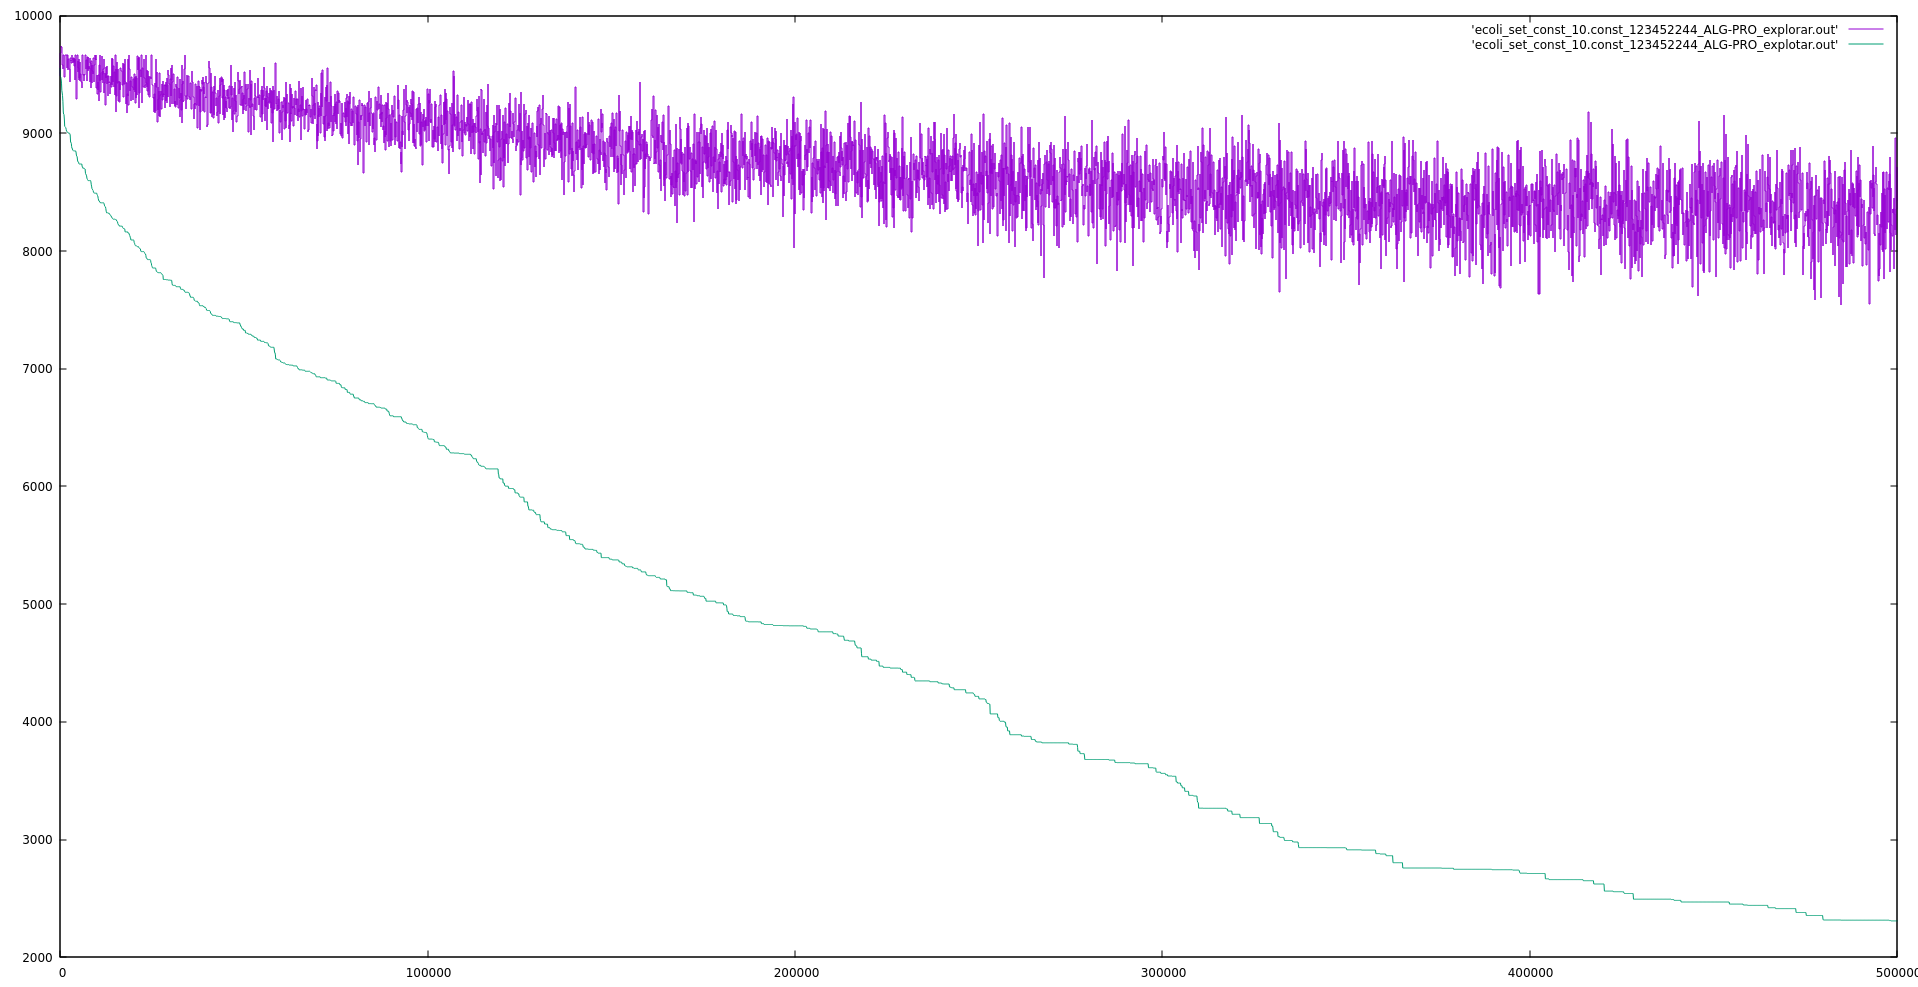
\includegraphics[scale = 0.33]{basico_sin_BL.png}
	
	\caption{Comportamiento de la primera versión de la propuesta.}
	\label{fig:basico_sin_BL}
\end{figure}

En esta imagen vemos en morado la mejor solución del conjunto de exploración y en verde la mejor solución del conjunto de explotación. Vemos como ambas poco a poco convergen, y tenemos que tener en  cuenta que el conjunto de exploración no alcanza buenas soluciones, porque en cuento logra encontrar una buena solución esta pasa al conjunto de explotación.

Vemos como claramente tenemos un problema de convergencia ya que incluso con medio millón de evaluaciones no llegamos a lograr que encuentre una solución aceptable, y seguramente con más evaluaciones siga encontrando nuevas soluciones.


\subsubsection{Mejora de la implementación: Mayor convergencia.}

Con el objetivo de paliar el problema de la convergencia demasiado lenta, decidí aplicar búsqueda local que implementé en la práctica 1 con pocas evaluaciones a la población de explotación. En principio esto soluciona el problema de convergencia, pero hace que se genere justo el problema contrario, existe demasiada convergencia y la búsqueda local requiere demasiadas evaluaciones, lo que hace que el algoritmo se pare de forma temprana y sin apenas explorar.

Para intentar paliar esto modifique la forma de aplicar la búsqueda local, ya no se aplicará al total de la población, si no solo a cierto porcentaje de esta, a las mejores soluciones que tenemos actualmente.


\begin{figure}[H]
	\centering
	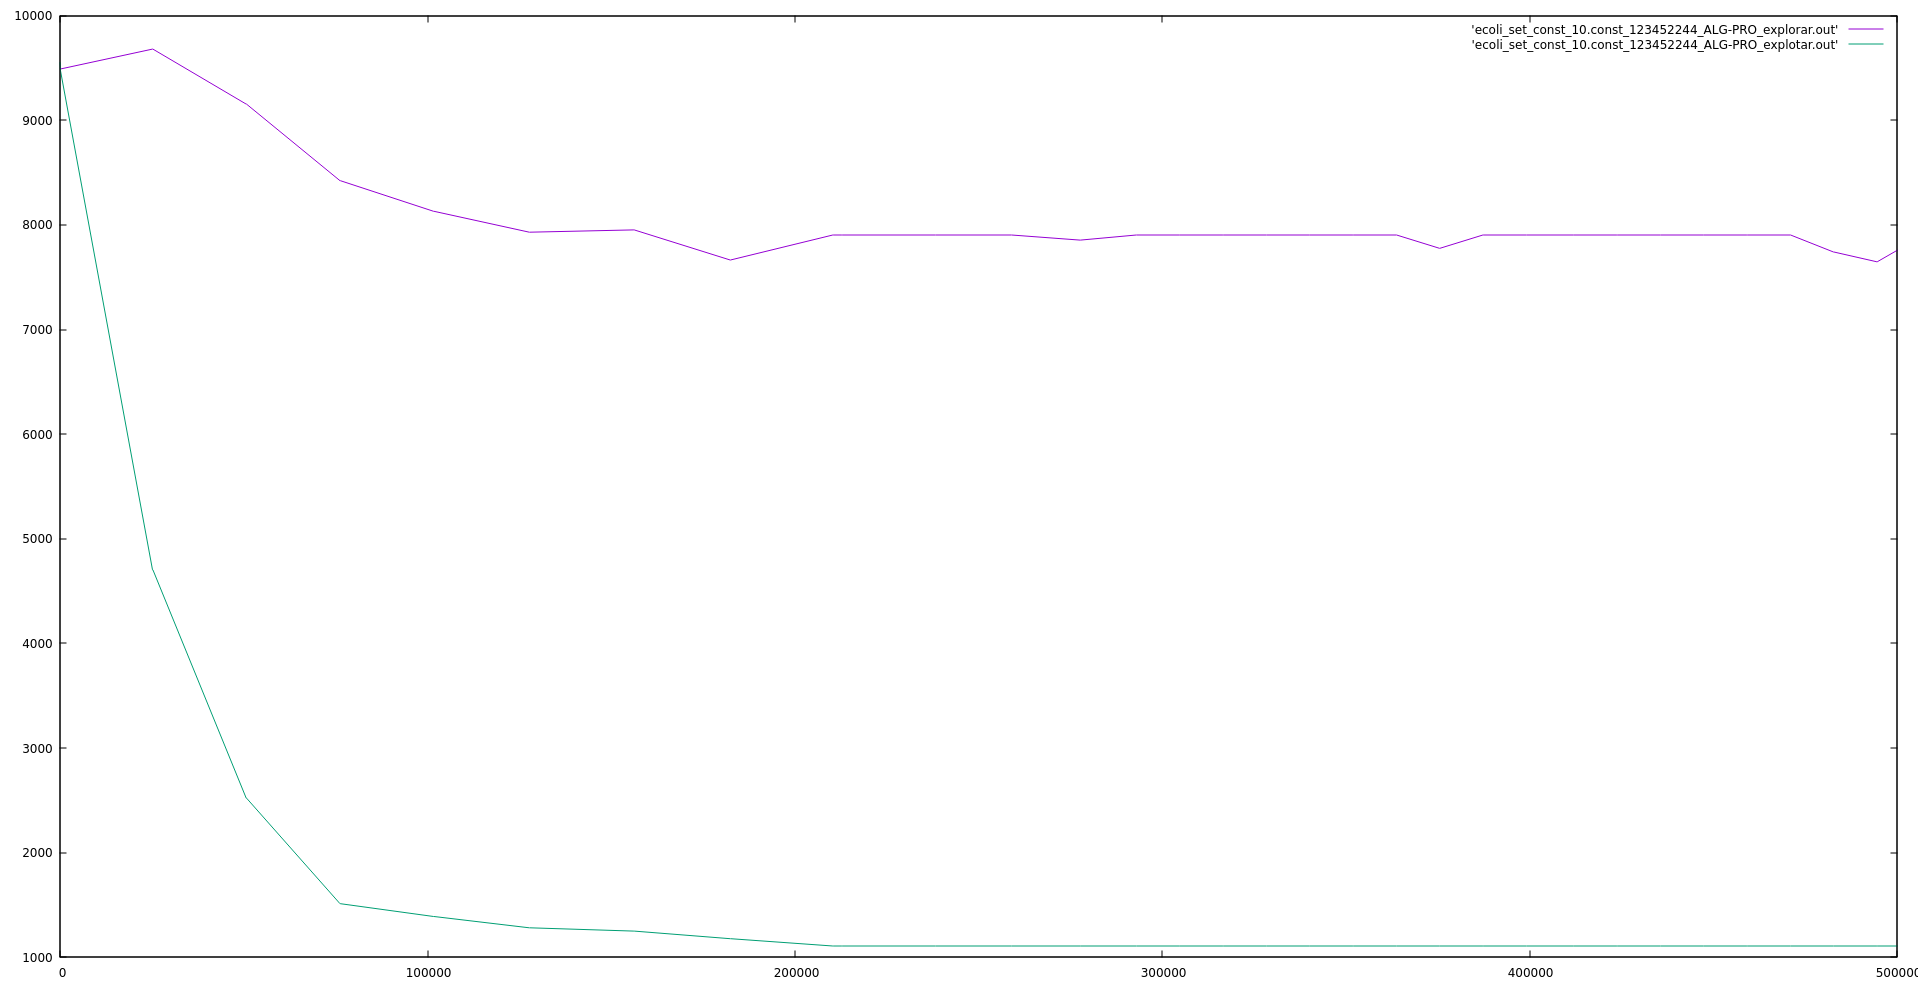
\includegraphics[scale = 0.33]{con_BL_explotar.png}
	
	\caption{Comportamiento de la segunda versión de la propuesta, con BL para converger.}
	\label{fig:basico_BL}
\end{figure}

Aun así vemos que esto sigue siendo demasiada explotación, y el algoritmo no se comporta como esperábamos, en el siguiente punto realizaremos los últimos ajustes y veremos como solucionar este problema.


\subsubsection{Mejora de la implementación y versión final: Ajuste de la convergencia y reinicialización de soluciones estancadas.}

Finalmente, una forma de hacer una mayor convergencia en el algoritmo pero sin que sea tan brusca como la búsqueda local ha sido utilizar la búsqueda local suave vista en la práctica 2 a las mejores soluciones de la población de explotación.

Esta solución ha dado un buen resultado, y además, debido a que una vez se estancaba la mejor solución, rápidamente toda la población de explotación acababa siendo una copia de esta solución he añadido una reinicialización de soluciones, cuando una solución de la población de explotación llega a ser la misma que la mejor solución encontrada, esta se desecha y la reemplazamos por una solución aleatoria. Con estas modificaciones conseguimos los siguientes resultados:


\begin{figure}[H]
	\centering
	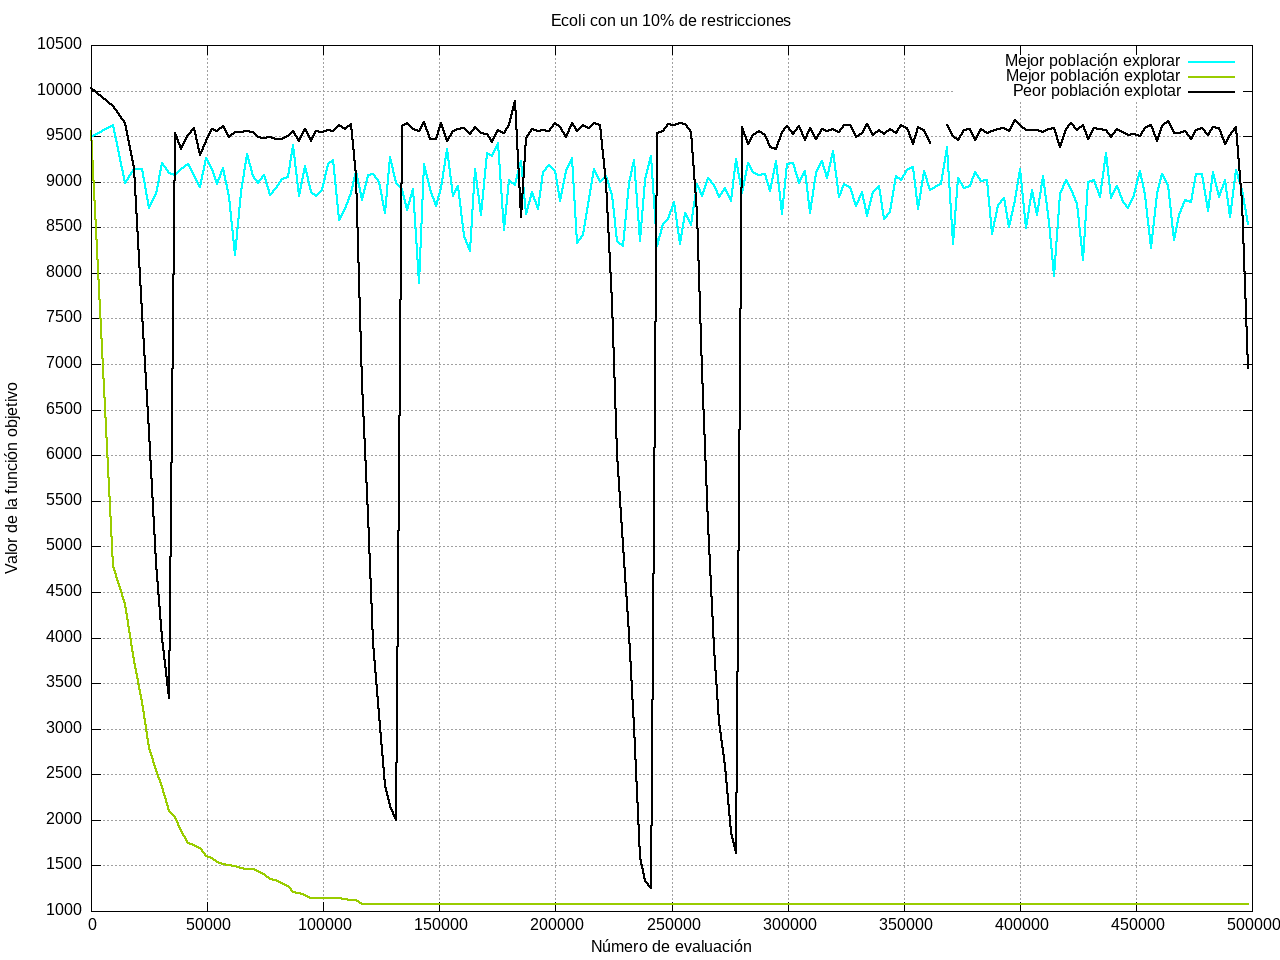
\includegraphics[scale = 0.50]{final_ecoli.png}
	
	\caption{Comportamiento de la versión final, con BL suave y reinicialización de soluciones.}
	\label{fig:final_ecoli}
\end{figure}

En esta gráfica, un poco distinta de las otras, vemos en verde la mejor solución de la población de explotación, en negro la peor de la población de explotación y en azul la mejor de la población de exploración.

Vemos como al principio del algoritmo, cuando todavía no ha logrado converger, se consigue reducir el valor de la función objetivo gracias al método de acercamiento de soluciones a la mejor, sumado a la exploración que nos da la segunda población, que como vemos, las mejores soluciones de exploración y las peores de explotación se intercambian de forma correcta. Vemos como en distintas ocasiones se encuentra un mínimo local, la solución se estanca y se reinicializa, o incluso mientras desciende se da el caso de que una solución llega a la mejor, de ahí el primer pico que encontramos en la peor solución del conjunto de explotación, ya que se cambia por una solución aleatoria cuando una llega a la misma que teníamos, y la nueva aleatoria con alta probabilidad va a ser muy mala solución, siendo la nueva peor. Esta reinicialización nos sirve para encontrar un nuevo mínimo más adelante, y a partir de ahí ya con mayor dificultad de encontrar una mejor solución ya que la actual es bastante buena, comienza a verse cada vez más reinicializaciones, fomentando la exploración cuando ya no puede explotar más.

De esta forma hemos conseguido equilibrar tanto la exploración como la explotación y se ha llegado a diseñar una metaheurística que es capaz de cambiar de estrategia dependiendo de la situación de las soluciones a las que llegue.

Esto se ha conseguido ya que tanto cada vez que se cambiaba de mejor solución como en los intercambios de información de las poblaciones, el resto de la población seguía manteniendo información sobre las mejores soluciones antiguas, y esto les llevaba a encontrar nuevas soluciones mejores. Una vez una solución gana peso sobre las demás y hace que todas las otras soluciones se estanquen en esa, se reinicializan con el objetivo de encontrar una solución distinta.


\subsection{Parámetros.}

Tras la explicación de como ha avanzado la propuesta original y como se ha adaptado para llegar a la versión final, finalmente el algoritmo contará con los siguientes parámetros:

\begin{enumerate}
	\item Máximo de evaluaciones: Este algoritmo tendrá como condición de parada el número de evaluaciones que le pasemos por parámetro.
	\item Tamaño de la población: El número de soluciones que tendremos en la población de explotar. El número de elementos de la población de explorar vendrá en función de este parámetro y otro que veremos más adelante.
	\item Probabilidad de modificar un gen: Esta probabilidad $p\_modificar\_gen$ será la probabilidad con la que se decidirá en cada elemento de una solución de la población de explotación si dicho elemento se sustituye por el de la mejor solución. Para la probabilidad de si alejarse de la mejor solución en la población de exploración usaremos $1 - p\_modificar\_gen$.
	\item Porcentaje explorar: Este porcentaje es el porcentaje de tamaño de la población de explorar con respecto al tamaño de la población de explotar. Si tiene valor $1$, ambas poblaciones son del mismo tamaño, si tiene valor $0.5$, la población de explorar tendrá la mitad de soluciones que la población de explotar.
	\item Porcentaje a intercambiar: Porcentaje de soluciones que se intercambian entre ambas poblaciones en cada iteración. Se intercambian las peores del conjunto de explotar por las mejores del conjunto de explorar.
	\item Porcentaje BL: Porcentaje de soluciones del conjunto de explotar a las que se le aplicará la búsqueda local suave. Se aplicará a las mejores soluciones.
	\item Salida: Parámetro por defecto a verdadero, con este controlaremos la salida de información a ficheros para luego obtener las gráficas del comportamiento del algoritmo. No se tendrá en cuenta en el pseudocódigo que presentaré, ya que es opcional.
\end{enumerate}

\newpage


\subsection{Pseudocódigo.}

Para este algoritmo usaremos la representación de un vector de enteros donde cada posición representa un elemento, de forma que el número que este en una posición indica el cluster al que asignamos ese elemento. Por ejemplo, si la posición 0 tiene un 1, quiere decir que el elemento 0 esta asignado al cluster 1.

Las soluciones se representan como una pareja de el vector con la asignación y el valor de la función objetivo.

El pseudocódigo final del algoritmo quedaría de la siguiente forma. Los argumentos son los explicados en el apartado anterior en orden. Todas las variables en el código son variables para operaciones auxiliares o bien para realizar la salida:

\begin{lstlisting}
Devuelve: Solución del PAR (pareja asignación y valoración)
Recibe:  MAX_EVALS
		 TAM_POB_INI
		 PROB_MOD_GEN
		 PORCENTAJE_EXPLORAR
		 PORCENTAJE_INTERCAMBIAR
		 PORCENTAJE_BL
		 
		 
	poblacion_explotar = generar_poblacion_aleatoria(TAM_POB_INI)
	poblacion_explorar = generar_poblacion_aleatoria(TAM_POB_INI * PORCENTAJE_EXPLORAR)
	
	mejor_explotar = indice_mejor_elemento(poblacion_explotar)
	
	evals = 0
	
	Mientras evals < MAX_EVALS:
		Para i = 0 hasta poblacion_explorar.size():
			Para cada elemento j de una solución:
				Si aleatorio(0,1) <= 1 - PROB_MOD_GEN:
					Modificamos la asignacion poblacion_explorar[i].asignacion[j] a una distinta a poblacion_explotar[mejor_explotar].asignacion[j]
					
			poblacion_explorar[i].valoracion = funcion_objetivo(poblacion_explorar[i].asignacion)
			evals++
		
		
		
		
		
		
		Para i = 0 hasta poblacion_explotar.size():
			Si i != mejor_explotar:
				Para cada elemento j de una solución:
					Si aleatorio(0,1) <= PROB_MOD_GEN
						poblacion_explotar[i].asignacion[j] = poblacion_explotar[mejor_explotar].asignacion[j]
						
				poblacion_explotar[i].valoracion = funcion_objetivo(poblacion_explotar[i].asignacion)
				evals++

				Si poblacion_explotar[i] == poblacion_explotar[mejor_explotar]
					poblacion_explotar[i] = generar_solucion_aleatoria()
					poblacion_explotar[i].valoracion = funcion_objetivo(poblacion_explotar[i].asignacion)
					evals++
					
					
				
				
			
			
		indices_mejores_explotar = bucar_indices_mejores(poblacion_explotar, TAM_POB_INI * PORCENTAJE_BL)
		
		Para todo i en indices_mejores_explotar:
			// la busqueda local suave devuelve las evaluaciones utilizadas			
			eval += algoritmo_BLS(poblacion_explotar[i])
			
			
		indices_mejores_explorar = buscar_indices_mejores(poblacion_explorar, TAM_POB_INI * PORCENTAJE_INTERCAMBIAR)
		
		indices_peores_explotar = buscar_indices_peores(poblacion_explotar, TAM_POB_INI * PORCENTAJE_INTERCAMBIAR)
		
		Intercambiamos las soluciones de ambas poblaciones usando los indices obtenidos
		
		mejor_explotar = indice_mejor_elemento(poblacion_explotar)

	Devolver poblacion_explotar[mejor_explotar]
			
\end{lstlisting}


\subsection{Parámetros escogidos para las ejecuciones.}





\section{Proceso de implementación.}

Para la implementación he desarrollado mis propias clases en C++, como adjunto en la carpeta de fuentes. Para las estructuras de datos he utilizado la STL:

\begin{itemize}
	\item Clase map para las restricciones.
	\item Clase vector para los datos y centroides
	\item Clase set para los elementos de los clusters
	\item Clase pair para almacenar las parejas de restricciones, así como para operaciones auxiliares.
\end{itemize}

Además de estas clases de C++ y las implementadas por mi explicadas a lo largo de este guión también he usado las funciones de generación de números aleatorios dadas por los profesores añadiendo algunas funciones, como por ejemplo generar un número aleatorio entre 0 y un número dado, de forma que el número generado N cumpla que 0 <= N entre otras.

También he utilizado las funciones dadas por los profesores de la asignatura para medir el tiempo.


\subsection{Manual de uso.}

En la carpeta del código fuente existe un fichero Markdown (se puede abrir como texto plano, pero recomiendo un lector de Markdown para facilitar la lectura, editores como Atom o VSCode tienen uno integrado) README.md en el que se explica toda la estructura del código, carpetas, etc.

En esta sección haré un resumen de esto con lo necesario para compilar y ejecutar el programa.

\subsubsection{Compilar:}

Para compilar el programa hay que moverse a la carpeta de fuentes, donde se encuentra el archivo \texttt{Makefile} y ejecutar:

\begin{lstlisting}
make
\end{lstlisting}

Esto nos generará en la carpeta \textit{bin/} el ejecutable.




\subsubsection{Ejecución:}

Podemos lanzar el programa con:

\begin{lstlisting}
./bin/practica1 <fichero_datos> <fichero_restricciones> <num_clusters> <semilla>
\end{lstlisting}

Cada ejecución del programa lanzará todos los algoritmos explicados en esa misma ejecución.

También cabe destacar que en la ruta del fichero de datos se creará un fichero con la extensión \texttt{.out} con la salida y solución del PAR, este fichero contendrá en su nombre la semilla con la que se ha ejecutado, el algoritmo y el conjunto de datos usado.

En la carpeta de gráficas encontraremos una serie de ficheros .gp con las que generaremos gráficas para los algoritmos de búsqueda local, algoritmos genéticos y enfriamiento simulado. También encontramos dos carpetas:

\begin{itemize}
	\item Carpeta datos: El programa automáticamente generará estos ficheros que usaremos de entrada para generar los gráficos.
	\item Carpeta salida\_png: Donde se generarán los gráficos.
\end{itemize}

Para generar los gráficos simplemente tenemos que ejecutar el programa y despues ejecutar \texttt{gnuplot <fichero>.gp} dentro de la carpeta gráficas para obtener los png.


Es importante ejecutar los algoritmos antes de intentar generar las gráficas.

\newpage




\section{Experimentos y análisis de resultados.}


\subsection{Descripción de los casos.}

En nuestro caso, para el problema del PAR trabajaremos sobre tres conjuntos de datos:

\begin{itemize}
	\item{Iris: Conjunto de datos sobre tres tipos de flores Iris. En este caso tendremos un conjunto de 150 datos y el objetivo será clasificar estas flores según su tipo.}
	\item{Ecoli: Conjunto de datos con características de células, empleadas para predecir la localización de proteínas. En total son 336 datos, de 8 clases distintas.}
	\item{Rand: Conjunto de datos artificial, formado por tres conjuntos de datos bien diferenciados generados a base de distribuciones normales. En total 150 datos con 3 clasificaciones distintas.}
	\item{Newthyroid: Conjunto de datos con medidas cuantitativas tomadas sobre la glándula tiroides de 215 pacientes con 3 clasificaciones distintas.}
\end{itemize}

Destacar que en nuestro problema las restricciones tendrán un papel muy importante, ya que los conjuntos de datos son muy distintos y estas restricciones son un añadido no original del problema, podría darse el caso de que dos elementos que en principio son de la misma clase estén separados por las restricciones, en caso de tener muy en cuenta las restricciones en nuestra función objetivo, o viceversa, es decir, que realice la asignación de clases sin tener en cuenta las restricciones si a estas no se les da la suficiente importancia.


\subsubsection{Semillas escogidas.}

Las semillas que voy a usar son:

\begin{itemize}
	\item {123452244}
	\item {9398429}
	\item {12321}
	\item {213566}
	\item {3939021}
\end{itemize}

\subsection{Teorema No Free Lunch}

Como hemos visto en teoría, las metaheurísticas son métodos de resolución genéricos que podemos aplicar a cualquier problema, y siguiendo el teorema de no free lunch, una metaheurística que se comporte bien en un tipo de problemas se comportará mal en el resto de problemas, luego los análisis que realizaré en este documento se centrarán exclusivamente en el Problema de Asignación con Restricciones, esto quiere decir que es muy probable que las metaheurísticas más adelante analizadas se comporten de manera distinta sobre otros problemas y por tanto este análisis no se podrá extrapolar a otros problemas.

\newpage

\subsection{Resultados obtenidos.}


\subsection{Análisis de resultados.	}


\subsubsection{10\% de restricciones.}


\subsubsection{20\% de restricciones.}


\subsection{Otros experimentos: Estudio de los parámetros de la metaheurística propuesta.}


\end{document}
